%----------------------------------------------------------------------------------------
%	PACKAGES AND OTHER DOCUMENT CONFIGURATIONS
%----------------------------------------------------------------------------------------

\documentclass[
11pt, % The default document font size, options: 10pt, 11pt, 12pt
%oneside, % Two side (alternating margins) for binding by default, uncomment to switch to one side
english, % ngerman for German
singlespacing, % Single line spacing, alternatives: onehalfspacing or doublespacing
%draft, % Uncomment to enable draft mode (no pictures, no links, overfull hboxes indicated)
%nolistspacing, % If the document is onehalfspacing or doublespacing, uncomment this to set spacing in lists to single
%liststotoc, % Uncomment to add the list of figures/tables/etc to the table of contents
%toctotoc, % Uncomment to add the main table of contents to the table of contents
%parskip, % Uncomment to add space between paragraphs
%nohyperref, % Uncomment to not load the hyperref package
headsepline, % Uncomment to get a line under the header
%chapterinoneline, % Uncomment to place the chapter title next to the number on one line
%consistentlayout, % Uncomment to change the layout of the declaration, abstract and acknowledgements pages to match the default layout
]{style} % The class file specifying the document structure

\usepackage[utf8]{inputenc} % Required for inputting international characters
\usepackage[T1]{fontenc} % Output font encoding for international characters

\usepackage{mathpazo} % Use the Palatino font by default

\usepackage[backend=bibtex,style=authoryear,natbib=true]{biblatex} % Use the bibtex backend with the authoryear citation style (which resembles APA)

\addbibresource{./misc/bibliography.bib} % The filename of the bibliography

\usepackage[autostyle=true]{csquotes} % Required to generate language-dependent quotes in the bibliography

\usepackage{hyperref}% http://ctan.org/pkg/hyperref

%----------------------------------------------------------------------------------------
%	MARGIN SETTINGS
%----------------------------------------------------------------------------------------

\geometry{
	paper=a4paper, % Change to letterpaper for US letter
	inner=2.5cm, % Inner margin
	outer=3.8cm, % Outer margin
	bindingoffset=.5cm, % Binding offset
	top=1.5cm, % Top margin
	bottom=1.5cm, % Bottom margin
	%showframe, % Uncomment to show how the type block is set on the page
}

%----------------------------------------------------------------------------------------
%	THESIS INFORMATION
%----------------------------------------------------------------------------------------

\thesistitle{Automated Malware Analysis Using Large Language Models} % Your thesis title, this is used in the title and abstract, print it elsewhere with \ttitle
\supervisor{Dr Robert G \textsc{Smith}} % Your supervisor's name, this is used in the title page, print it elsewhere with \supname
\examiner{} % Your examiner's name, this is not currently used anywhere in the template, print it elsewhere with \examname
\degree{M.Sc} % Your degree name, this is used in the title page and abstract, print it elsewhere with \degreename
\author{Andre M M \textsc{Faria}} % Your name, this is used in the title page and abstract, print it elsewhere with \authorname
\addresses{Dublin, Ireland} % Your address, this is not currently used anywhere in the template, print it elsewhere with \addressname

\subject{Applied Cybersecurity} % Your subject area, this is not currently used anywhere in the template, print it elsewhere with \subjectname
\keywords{} % Keywords for your thesis, this is not currently used anywhere in the template, print it elsewhere with \keywordnames
\university{\href{https://www.tudublin.ie/}{Technological University Dublin}} % Your university's name and URL, this is used in the title page and abstract, print it elsewhere with \univname
\department{\href{https://www.tudublin.ie/explore/faculties-and-schools/computing-digital-data/informatics-and-cybersecurity/}{School of Informatics and Cyber Security}} % Your department's name and URL, this is used in the title page and abstract, print it elsewhere with \deptname
\submitdate{May 2025} % The month and year that you submit your FINAL draft to the university, this is not currently used anywhere in the template, print it elsewhere with \subdate

\AtBeginDocument{
\hypersetup{pdftitle=\ttitle} % Set the PDF's title to your title
\hypersetup{pdfauthor=\authorname} % Set the PDF's author to your name
\hypersetup{pdfkeywords=\keywordnames} % Set the PDF's keywords to your keywords
}

\begin{document}

\frontmatter % Use roman page numbering style (i, ii, iii, iv...) for the pre-content pages

\pagestyle{plain} % Default to the plain heading style until the thesis style is called for the body content

%----------------------------------------------------------------------------------------
%	TITLE PAGE
%----------------------------------------------------------------------------------------

\begin{titlepage}
	\begin{center}

		\vspace*{.06\textheight}
		{\scshape\LARGE \univname\par}\vspace{1.5cm} % University name
		\textsc{\Large Masters Thesis}\\[0.5cm] % Thesis type

		\HRule \\[0.4cm] % Horizontal line
		{\huge \bfseries \ttitle\par}\vspace{0.4cm} % Thesis title
		\HRule \\[1.5cm] % Horizontal line

		\begin{minipage}[t]{0.4\textwidth}
			\begin{flushleft} \large
				\emph{Author:}\\
				\href{https://www.linkedin.com/in/andremmfaria/}{\authorname} % Author name - remove the \href bracket to remove the link
			\end{flushleft}
		\end{minipage}
		\begin{minipage}[t]{0.4\textwidth}
			\begin{flushright} \large
				\emph{Supervisor:} \\
				\href{https://www.tudublin.ie/explore/faculties-and-schools/computing-digital-data/informatics-and-cybersecurity/people/academic-staff/robertsmith.php}{\supname} % Supervisor name - remove the \href bracket to remove the link
			\end{flushright}
		\end{minipage}\\[2cm]

		\vfill

		\large \textit{A thesis submitted in fulfillment of the requirements\\ for the degree of \degreename\\ in \subjectname}\\[0.4cm] % University requirement text
		\textit{in the}\\[0.4cm]
		\deptname\\[2cm] % Research group name and department name

		
\includegraphics[width=0.2\textwidth]{./image/uni-logo.png} % University/department logo - uncomment to place it

		\vfill

		{\large \subdate}\\[4cm] % Date

		\vfill
	\end{center}
\end{titlepage}

%----------------------------------------------------------------------------------------
%	DECLARATION PAGE
%----------------------------------------------------------------------------------------

\begin{declaration}
	\addchaptertocentry{\authorshipname} % Add the declaration to the table of contents
	\noindent I, \authorname, declare that this thesis titled, \enquote{\ttitle} and the work presented in it are my own. I confirm that:

	\begin{itemize}
		\item This work was done wholly or mainly while in candidature for a research degree
		      at this Institute of Technology Blanchardstown.
		\item Where any part of this thesis has previously been submitted for a degree or any
		      other qualification at this University or any other institution, this has been
		      clearly stated.
		\item Where I have consulted the published work of others, this is always clearly
		      attributed.
		\item Where I have quoted from the work of others, the source is always given. With
		      the exception of such quotations, this thesis is entirely my own work.
		\item I have acknowledged all main sources of help.
		\item Where the thesis is based on work done by myself jointly with others, I have
		      made clear exactly what was done by others and what I have contributed
		      myself.\\
	\end{itemize}

	\noindent Signed:\\
	\rule[0.5em]{25em}{0.5pt} % This prints a line for the signature

	\noindent Date: \today \\
	\rule[0.5em]{25em}{0.5pt} % This prints a line to write the date
\end{declaration}

\cleardoublepage

%----------------------------------------------------------------------------------------
%	QUOTATION PAGE
%----------------------------------------------------------------------------------------

\vspace*{0.2\textheight}

\noindent\enquote{\itshape The true thesis are the friends we make along the way.}\bigbreak

\hfill Anonymous

%----------------------------------------------------------------------------------------
%	ABSTRACT PAGE
%----------------------------------------------------------------------------------------

\begin{abstract}
	\addchaptertocentry{\abstractname} % Add the abstract to the table of contents
	Despite the fact that an abstract is quite brief, it must do almost as much
	work as the multi-page paper that follows it. In a computer science paper, this
	means that it should in most cases include the following sections. Each section
	is typically a single sentence, although there is room for creativity. In
	particular, the parts may be merged or spread among a set of sentences. Use the
	following as a checklist for your next abstract (URL:
	http://www.ece.cmu.edu/~koopman/essays/abstract.html):

	\begin{description}
	\item[Motivation:] Why do we care about the problem and the results? If the problem
			isn't obviously "interesting" it might be better to put motivation first; but
			if your work is incremental progress on a problem that is widely recognized as
			important, then it is probably better to put the problem statement first to
			indicate which piece of the larger problem you are breaking off to work on.
			This section should include the importance of your work, the difficulty of the
			area, and the impact it might have if successful.
	\item[Problem statement:] What problem are you trying to solve? What is the scope of
			your work (a generalized approach, or for a specific situation)? Be careful not
			to use too much jargon. In some cases it is appropriate to put the problem
			statement before the motivation, but usually this only works if most readers
			already understand why the problem is important.
	\item[Approach:] How did you go about solving or making progress on the problem? Did
			you use simulation, analytic models, prototype construction, or analysis of
			field data for an actual product? What was the extent of your work (did you
			look at one application program or a hundred programs in twenty different
			programming languages?) What important variables did you control, ignore, or
			measure?
	\item[Results:] What's the answer? Specifically, most good computer architecture
			papers conclude that something is so many percent faster, cheaper, smaller, or
			otherwise better than something else. Put the result there, in numbers. Avoid
			vague, hand-waving results such as "very", "small", or "significant." If you
			must be vague, you are only given license to do so when you can talk about
			orders-of-magnitude improvement. There is a tension here in that you should not
			provide numbers that can be easily misinterpreted, but on the other hand you
			don't have room for all the caveats.
	\item[Conclusions:] What are the implications of your answer? Is it going to change
			the world (unlikely), be a significant "win", be a nice hack, or simply serve
			as a road sign indicating that this path is a waste of time (all of the
			previous results are useful). Are your results general, potentially
			generalizable, or specific to a particular case?

	\end{description}
\end{abstract}

%----------------------------------------------------------------------------------------
%	ACKNOWLEDGEMENTS
%----------------------------------------------------------------------------------------

\begin{acknowledgements}
	\addchaptertocentry{\acknowledgementname} % Add the acknowledgements to the table of contents
	The acknowledgments and the people to thank go here, don't forget to include your project advisor\ldots
\end{acknowledgements}

%----------------------------------------------------------------------------------------
%	LIST OF CONTENTS/FIGURES/TABLES PAGES
%----------------------------------------------------------------------------------------

\tableofcontents % Prints the main table of contents

\listoffigures % Prints the list of figures

\listoftables % Prints the list of tables

%----------------------------------------------------------------------------------------
%	ABBREVIATIONS
%----------------------------------------------------------------------------------------

\begin{abbreviations}{ll} % Include a list of abbreviations (a table of two columns)

	\textbf{LAH} & \textbf{L}ist \textbf{A}bbreviations \textbf{H}ere\\
	\textbf{WSF} & \textbf{W}hat (it) \textbf{S}tands \textbf{F}or\\

\end{abbreviations}

%----------------------------------------------------------------------------------------
%	PHYSICAL CONSTANTS/OTHER DEFINITIONS
%----------------------------------------------------------------------------------------

\begin{constants}{lr@{${}={}$}l} % The list of physical constants is a three column table

	% The \SI{}{} command is provided by the siunitx package, see its documentation for instructions on how to use it

	Speed of Light & $c_{0}$ & \SI{2.99792458e8}{\meter\per\second} (exact)\\
	%Constant Name & $Symbol$ & $Constant Value$ with units\\

\end{constants}

%----------------------------------------------------------------------------------------
%	SYMBOLS
%----------------------------------------------------------------------------------------

\begin{symbols}{lll} % Include a list of Symbols (a three column table)

	$a$ & distance & \si{\meter} \\
	$P$ & power & \si{\watt} (\si{\joule\per\second}) \\
	%Symbol & Name & Unit \\

	\addlinespace % Gap to separate the Roman symbols from the Greek

	$\omega$ & angular frequency & \si{\radian} \\

\end{symbols}

%----------------------------------------------------------------------------------------
%	DEDICATION
%----------------------------------------------------------------------------------------

\dedicatory{For/Dedicated to/To my\ldots}

%----------------------------------------------------------------------------------------
%	THESIS CONTENT - CHAPTERS
%----------------------------------------------------------------------------------------

\mainmatter % Begin numeric (1,2,3...) page numbering

\pagestyle{thesis} % Return the page headers back to the "thesis" style

% Include the chapters of the thesis as separate files from the Chapters folder
% Uncomment the lines as you write the chapters

%----------------------------------------------------------------------------------------

% Define some commands to keep the formatting separated from the content 
\newcommand{\keyword}[1]{\textbf{#1}}
\newcommand{\tabhead}[1]{\textbf{#1}}
\newcommand{\code}[1]{\texttt{#1}}
\newcommand{\file}[1]{\texttt{\bfseries#1}}
\newcommand{\option}[1]{\texttt{\itshape#1}}

%----------------------------------------------------------------------------------------

% Chapter 1

\chapter{Introduction and Background}
\label{sec:introduction}

\label{Chapter1} % For referencing the chapter elsewhere, use \ref{Chapter1} 

\section{Before You Begin}
!!IMPORTANT!!: before you begin this research, be sure that you are familiar with the University's policy on Academic Integrity: \url{https://www.tudublin.ie/explore/about-the-university/academic-affairs/academic-quality-assurance-and-enhancement/academic-integrity/}

Also, read the important advice on receiving Feedback, Proofreading and the use
of Writing Assistants in Appendix \ref{app:feedback}, \ref{app:proofreading} \&
\ref{App:writing_assist}.

\section{Section Introduction}
%always begin a section with an introduction and end it with a summery
A thesis is built up of a series of chapters that construct a substantiated and
convincing response to the research question(s). Typically, a thesis contains
the following chapters: an introduction; a literature review; a description of
methodology; a report and discussion of results; and a conclusion. A thesis may
have five to eight chapters depending on the nature of the study, the required
word count and the requirements of the degree.

\subsection{About the Introduction Chapter}
An introduction is crucial to setting the tone of your thesis – it is the first
impression you’ll make on your readers (assessors). Briefly, it presents the
purpose, context and scope of your research. Likewise, a conclusion is just as
crucial – it is the lasting impression you’ll make on your readers (assessors).
Not only does it give a summary of your thesis, but should provide a clear,
convincing answer to your research question(s).
\subsection{Subsection header 2}
After introducing your work, you should list your research questions,
hypothesis, and objectives.

Always keep in mind the meaning of the word ``\textit{Thesis}''. That is: a
thesis is a statement or theory that is put forward as a premise to be
maintained or proved. A Hypo\textit{thesis} then, is a sub-thesis, or a smaller
part of the overarching thesis.

All of your research questions must aim to prove or disprove your thesis.. and
thus your hypotheses.

See more here: \url{https://www.statconsul.com/research-questions.php}
\subsection{Subsection header 3}
The last thing you do in an Introduction Chapter is to outline the contents of
your thesis, i.e., a review of then literature is provided in Chapter
\ref{sec:LitReview}, starting with... etc... Chapter \ref{sec:Method} provides
a description of the method... etc...

\vfill
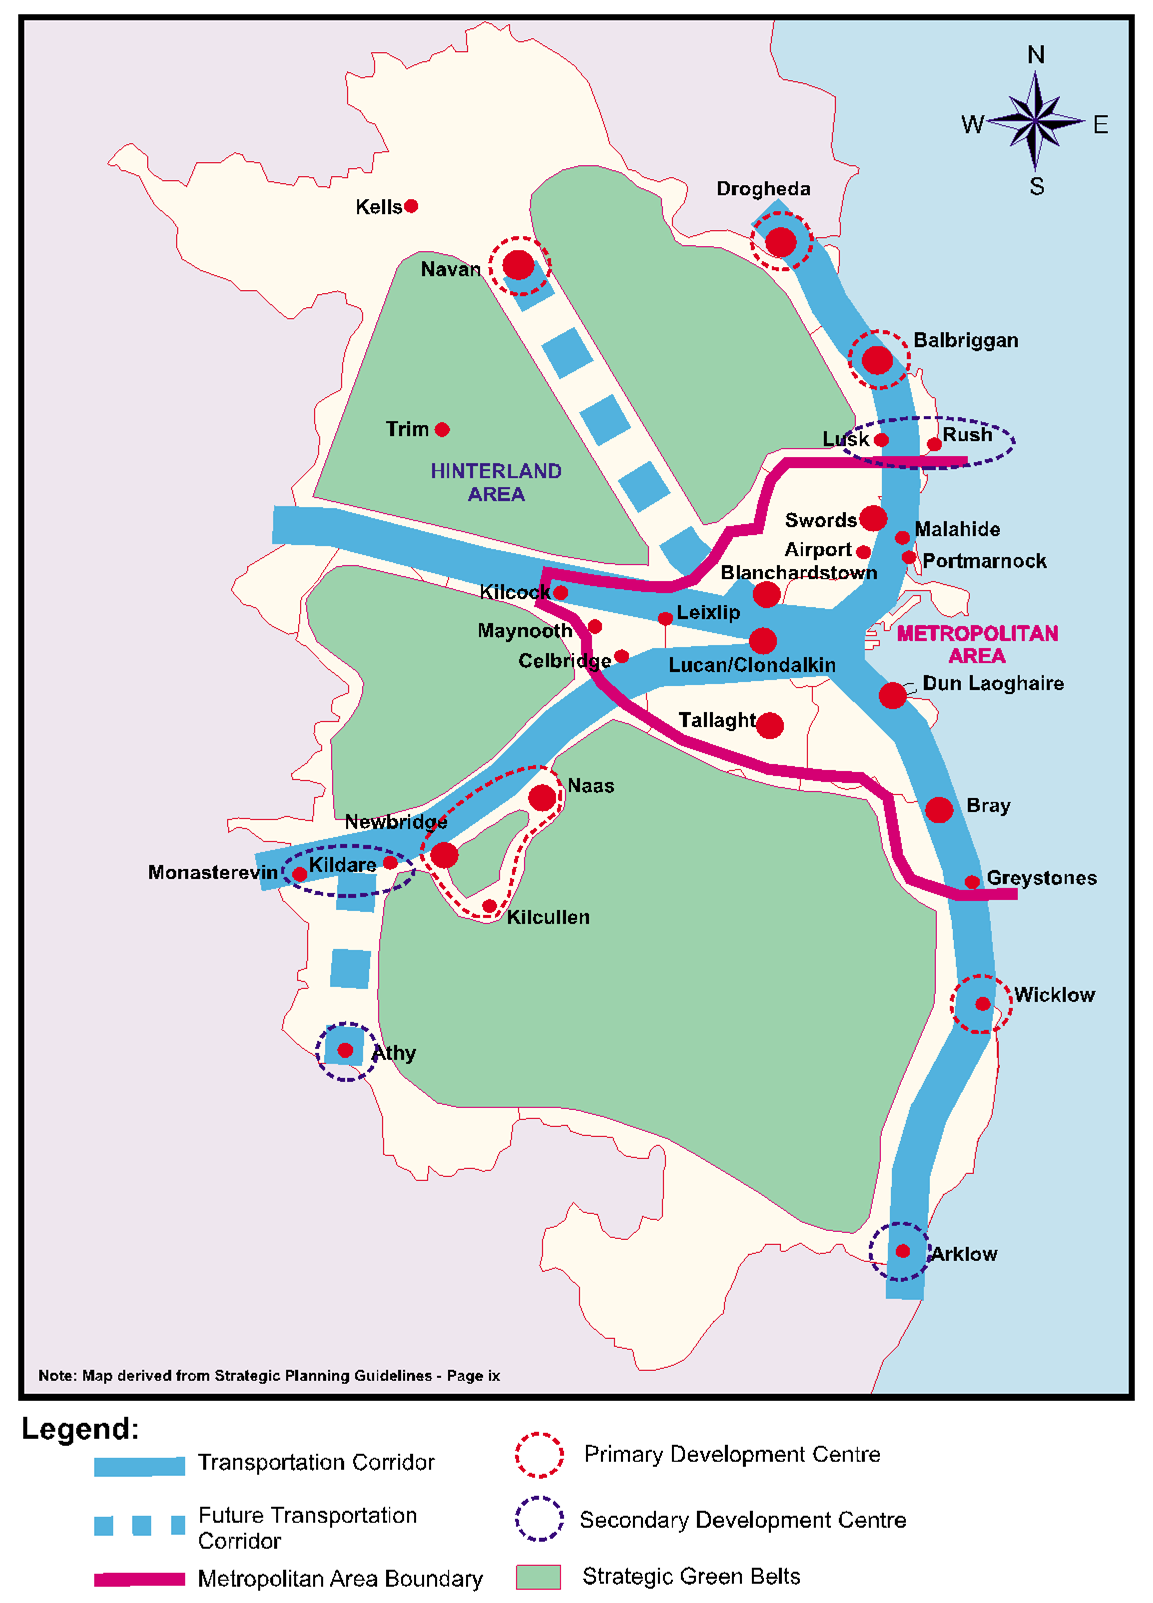
\includegraphics[width=\textwidth]{intro1.png}
\vfill

\section{More about the Introduction chapter}
The introduction allows you to orient the reader to your research project and
preview the organisation of your thesis. In the introduction, state what the
topic is about, explain why it needs to be further researched and introduce
your research question(s) or hypothesis.

Whilst patterns of organisation in introductions vary, there are some common
features that will help you to achieve an informative and engaging
introduction. Let’s identify these features:

\begin{itemize}
	\item Introduce the topic
	\item Define key terms and concepts
	\item Give background and context for the topic (this may include a brief literature
	      review)
	\item Review and evaluate the current state of knowledge in the topic (this may
	      include a brief literature review)
	\item Identify any gaps, shortcomings and problems in the research to date
	\item Introduce your research question(s) or hypothesis
	\item Briefly describe your methodology and/or theoretical approach
	\item Explain the aim of your research and what contribution it will make to the
	      topic
	\item Give an overview of the chapter outline of the thesis.
\end{itemize}

It’s important to note that, depending on your field of study and the faculty
requirements of your thesis, not all of these features will be relevant. Also,
these features may occur in varied orders.

Most people write many drafts of their introduction. It can be useful to write
one early in the research process to clarify your thinking. You will need to
write a version for your confirmation proposal and other milestones. As your
research progresses and your ideas develop, you will need to revise it. When
the final draft of chapters is complete, check the introduction once more to
make sure that it accurately reflects what you have actually done.

% Chapter 2

\chapter{Literature Review}
\label{sec:LitReview}

\label{Chapter2} % For referencing the chapter elsewhere, use \ref{Chapter2} 

\section{What is a Literature Review?}
A literature review is a section of your thesis or dissertation in which you
discuss previous research on your subject. Following your Introduction chapter,
your literature review begins as you try to answer your larger research
question: Who has looked at what, why, and what have they found? It allows you
to understand what others have said about your topic, to verify your
assumptions, to refine your initial research question, and to identify gaps.
For your readers, the literature review also demonstrates that you are
knowledgeable about related research and scholarly traditions in your field.

\subsection{Preparing to Write}
The literature review is more than just a list of previous research papers in
the field. If you think of writing a thesis or dissertation as writing a story
of your research, the literature review then will be a story within a story. In
the literature review story, you tell the reader about general trends,
traditions, and approaches to your subject, ones that surround and support your
study.

Choose texts to help you try to answer your research question. As you explore
the literature, take notes:
\begin{itemize}
	\item Why did you pick up this text? [Reminder: What is being studied, by whom, why?
	      What did they find? As you pick up a text, note all documentation information.]
	\item How does this article, chapter, book, study help you answer your question or
	      not?
	\item When you find a publication of interest, read the Abstract to see if it is what
	      you are looking for. If not, discard the text. If it does seem to be what you
	      are looking for, then glance over the Introduction and Conclusions. Again, if
	      it is what you are looking for, you can now invest the time to read the entire
	      publication, or the section of the publication that interests you. This method
	      save a lot of time in the long term.
	\item Be sure that all publications are from a credible source: You can gauge this by
	      where an article/book has been published, if it has been peer reviewed, how it
	      has ben written, how many times it has been cited etc...
\end{itemize}

After you have read and written, draw a diagram, chart, or matrix that would
help you to visualize connections between your sources and reveal a possible
structure for your literature review. Some researcher like to print papers and
organise content with colour (with highlighters and post-it notes), others like
to use tools such as \textit{NVivo}. This approach allows you to notice
distinct patterns in the literature, e.g., how an algorithm has developed over
time. You may choose to plot it out on a timeline. Or, you may decide to
organize your literature review by the researchers' stance towards your
subject. Or, you may want to create a sort of bubble map to discover:
\begin{itemize}
	\item What major trends and patterns in the results of previous studies emerge?
	\item What common threads do you find?
	\item How do these studies connect?
\end{itemize}
There is no right or wrong way for structuring the review. It should explain the thinking process behind your choices and help reveal the need to answer your question (to fill a gap) and how to
go about doing that (the methodology).

When you have a rough draft completed, ask yourself:
\begin{itemize}
	\item What previous research has been more significant and less significant?
	\item What gaps in literature have you noticed? Why do these gaps exist?
	\item How might your research hypothesis or research questions inform your
	      organization and characterization of the previous literature?
\end{itemize}

\subsection{Revising}
When describing, critiquing, and citing your sources, use the following
citation patterns to introduce and comment on sources:
\begin{itemize}
	\item Generalisation (combining 2 or more sources): Describe what makes this group of
	      sources a category
	\item Summarise each key source; paraphrase the author[s]' argument (this is not
	      plagiarism because you are citing the work).
	\item Try to avoid using quotations to note key words or phrases... better not to
	      overuse this strategy and to use your own words where possible.
	\item Use block quotations (more than 40 words) sparingly.
\end{itemize}

\textit{However, avoid ambiguous citations like these two:}

In the example above, it is not clear whether Clement and Lee are major
researchers in their fields or what their work includes. Also, one author does
not suggest “wide investigation” or “much” research. Best to use multiple
sources for broad statements like these.

Help your readers make their way through your literature review by referring to
its organization or back to a part of the review, or by providing a definition.
For example, use words and phrases, such as \textit{In this section, I will
	discuss ...\\ This part will describe ...\\ For the purpose of this discussion,
	metadiscourse means ...\\ The main purpose of this review has been ...\\ Thus
	far, this review has outlined ...\\}

Things to Remember
\begin{itemize}
	\item Avoid describing each piece of relevant research in detail, piece by piece.
	\item Focus on general trends and approaches.
	\item Only critique the few most relevant, seminal sources. There is no need to
	      critique each source.
	\item When reviewing a study, avoid reporting an author’s assertions as though they
	      were findings.
	\item Highlight agreement before disagreement.
	\item Depending on your field of study, you may want to tell a story that led you to
	      this research and would help explain your choices to include or exclude
	      previous research.
\end{itemize}

\subsection{Sources}
They Say/I Say: The Moves That Matter in Academic Writing by Gerald Graff and
Cathy Birkenstein Academic Writing for Graduate Students and Telling a Research
Story: Writing a Literature Review by Christine B. Feak and John M Swales

\url{https://www.jsums.edu/wrightcenter/files/2016/03/Writing-a-Literature-Review.pdf}

\subsection{Citing and Referencing}

This Latex template uses the 'natbib' package to manage references and
citations. There is a good introduction to this package here:
\url{https://www.overleaf.com/learn/latex/Bibliography_management_with_natbib}

Note: there are different referencing styles, these can be set in the main
thesis.tex file. Find out which style you should use from your project
documentation, project coordinator or supervisor.

It is important to note that when referencing in-text, you should format the
citation differently depending on how you reference the author. Consider the
following sentence:

\begin{flushleft}
	``\textit{\cite{Smith2023PhD} explores the use of Association Rules Mining to identify patterns in a sign language dataset.}''
\end{flushleft}

You will note that when Smith's 2023 publication is referenced directly in the
text, only the year of the publication is in brackets, i.e., the authors name
is not in brackets.

\begin{flushleft}
	``\textit{The use of Association Rules Mining to identify patterns in a sign language dataset has been explored recently \citep{Smith2023PhD} .}''
\end{flushleft}

When the same publication is referenced indirectly at the end of the sentence,
the authors name and year of publication are inside the brackets. See the
following reference sheet to help you keep track of this:
\url{https://gking.harvard.edu/files/natnotes2.pdf}
 
% Chapter 3

\chapter{Methodology}
\label{sec:Method}

\label{Chapter3} % For referencing the chapter elsewhere, use \ref{Chapter3} 

\section{What is a Methodology?}
Every thesis, regardless of the discipline and field of inquiry it relates to,
needs to answer these questions:

\begin{itemize}
	\item How did you do your research?
	\item Why did you do it that way?
\end{itemize}

This covers not only the methods used to collect and analyse data, but also the
theoretical framework that informs both the choice of methods and the approach
to interpreting the data. In some disciplines, the approach to knowledge
underpinning both the type of research questions asked and the methods chosen
to answer them is called “methodology”, and needs to be articulated. Both
methods and theoretical approach relate explicitly to the research question(s)
addressed in the thesis.

You may need to summarise available methods and theoretical approaches for your
research topic; you will certainly need to justify your choice of method(s). If
you apply a combination of methods you’ll need to justify why you chose such an
approach. Your explanation should also indicate any reliability or validity
issues concerning the data, and discuss any ethical considerations that arise
from your choices.

Whilst patterns of organisation in a methods chapter may vary, there are some
common elements that you’ll need to include to achieve an informative chapter.
Let’s identify these features:

\begin{itemize}
	\item place or setting of the research
	\item duration of the study and other time related factors
	\item study design – e.g. an outline of the research stages including instruments and
	      techniques
	\item specifics of the participants, materials, etc.
	\item sampling frameworks (e.g. criteria, size, scope, etc.)
	\item any inclusions/exclusions
	\item outcome measurement procedures (e.g. statistical tests, comparisons, etc.)
	\item consent and ethics committee approval
	\item theoretical basis of the research
	\item data management
\end{itemize}

While most of these elements will be relevant to your methods chapter, you’ll
find that there are discipline specific elements and requirements. The detail
and emphasis of what is covered in a discussion of methods/methodology will be
different in different disciplines.

\subsection{STEM specific Method Chapter}
Key features of method descriptions in STEM disciplines include:

\begin{itemize}
	\item demonstration of fit between methods chosen and research question(s)
	\item rationale for choosing materials, methods and procedures
	\item details of materials, equipment and procedures that will allow others to:
	      \begin{itemize}
		      \item replicate experiments
		      \item understand and implement technical solutions
	      \end{itemize}
\end{itemize}

% Chapter 4

\chapter{Discussion of Results}
\label{sec:Results}

\label{Chapter4} % For referencing the chapter elsewhere, use \ref{Chapter4} 

\section{Section Introduction}

The reporting and discussion thesis chapters deal with the central part of the
thesis. This is where you present the data that forms the basis of your
investigation, shaped by the way you have interpreted it and developed your
argument or theories about it. In other words, you tell your readers the
research story that has emerged from your findings. These chapters will form
the bulk of your complete thesis. Before you even begin writing up the
reporting and discussion chapters, you’ll need to undertake some thinking and
planning.

There is quite a loot to say about this topic so Ive provided a like here for
further reading:
\url{https://www.monash.edu/student-academic-success/excel-at-writing/how-to-write/thesis-chapter/reporting-and-discussion-thesis-chapters}
 
% Chapter 5

\chapter{Conclusion}
\label{sec:Conclusion}

\label{Chapter5} % For referencing the chapter elsewhere, use \ref{Chapter5} 

\section{About Conclusions}
Depending on the type of research presented in the thesis, conclusion chapters
or sections tend to include at least some of the following:

\begin{itemize}
	\item A clear answer to your research question or hypothesis
	\item Summary of the main findings or argument
	\item Connections between your findings or argument to other research
	\item Explanation and significance of the findings
	\item Implications of the findings
	\item Limitations of the research and methodology
	\item Recommendations for future research
\end{itemize}

Your conclusion chapter is the place to emphasise the new knowledge that you’ve
contributed to the field of study and explain its significance. This chapter is
your opportunity to leave a strong impression on the reader (assessors) about
the strength and relevance of your research, and your skills as a researcher.

Importantly, the conclusion chapter must link with your introduction chapter to
complete the framing of the thesis and demonstrate that you have achieved what
you set out to do.
 

%----------------------------------------------------------------------------------------
%	THESIS CONTENT - APPENDICES
%----------------------------------------------------------------------------------------

\appendix % Cue to tell LaTeX that the following "chapters" are Appendices

% Include the appendices of the thesis as separate files from the Appendices folder
% Uncomment the lines as you write the Appendices

\appendix

\chapter{Frequently Asked Questions} % Main appendix title

\label{Appendix} % For referencing this appendix elsewhere, use \ref{Appendix}

\section{Getting Feedback}
\label{app:feedback}

\begin{enumerate}
	\item Get feedback \textbf{often} and from different audiences – your family,
	      friends, professors, colleagues, advisor, other graduate students. The more you
	      talk about your research, the more comfortable you get with it.
	\item Keep a positive attitude. Research is hard. If it were easy, everyone would be
	      doing it.
	\item Consider setting up or joining a thesis group to share your ideas and
	      experiences.
\end{enumerate}

\textbf{Supervisor's feedback}\\
Some supervisors will ask for you to send each chapter as you complete it, offering feedback at that point, and then again at the end when the thesis chapters are collated. Other supervisors may want to be more involved, and there are others who will not want to see your thesis until it is completed by your standards. Whichever approach your supervisor takes, be aware that they will need some time to read through your work and provide feedback. Your thesis review is likely not the only piece of work your supervisor is undertaking, so be patient and factor review time into your work schedule.

A couple of points to note about supervisor feedback:
\begin{itemize}
	\item You will receive feedback on your approach to research (i.e., method,
	      experiment design etc...) as well as your writing. It is your responsibility to
	      take notes at meetings etc. in order to record this feedback. It is also up to
	      you whether or not you act upon the feedback provided.
	\item Your supervisor's role is to guide your work. It is not their job to complete
	      the research, suggest methods, design experiments, or to write/rewrite sections
	      of your thesis.
	\item Your supervisor should be supportive but sometimes their feedback may be
	      difficult to hear. Just remember, their goal is to guide you and to make you a
	      better researcher. Learn to have your work criticised in a constructive manner,
	      it is part of the learning process.
	\item It is not the role of your supervisor to proofread your thesis. Many
	      supervisors will point out typos, grammatical errors or styling issues etc.
	      when they see them, but this is not their role.
\end{itemize}
\newpage

\section{Proofreading/copyediting} \label{app:proofreading}
It is important to have your work proofread\footnote{Two types of editing that
	are commonly used interchangeably are copy editing and proofreading. Both types
	of editing clean up writing, but each has its distinct contribution to the
	process.
	\url{https://thesiswhisperer.com/2016/11/30/doing-a-copy-edit-of-your-thesis/}}.
If English is not your first language, this is even more important for you.

\textbf{How?}\\
A good approach is to proofread yourself as you write and then again when you are finished writing a section or chapter. When you have a near final draft, have it proofread by a friend, family member, colleague, or a classmate etc... (not your supervisor). Choose your proofreader wisely. Make sure that they have good written English skills and are able to spot grammatical errors. A native English speaker can be good for this but not all native English speakers have the skills needed to be a good proofreader.

There are many things to look out for when reviewing your own work, everything
from text alignment and section numbering, to figures and tables, to spelling
and grammar. It's best to identify and fix any of these errors immediately.
Don't wait until the end because these will build up and it often takes longer
than you think to fix them.

If you find that you make the same mistake regularly, e.g., you misspell the
same word regularly, or you use a colon where you shouldn't, then make a list
of these to check back when you are finished each section (the search feature
is good for this).

\newpage
\section{Writing Assistants} \label{App:writing_assist}
In the past, students may have used tools such as Grammarly or Quetext, but
this has become more problematic because such editing tools now come with AI
assisted writing (see more here:
\url{https://tudublin.libguides.com/c.php?g=720901&p=5233062}).

Using tools such as a spell checker, a grammar checker, and a punctuation
checker are generally acceptable. Using more advanced tools to rewrite
sentences, check tone, offer alternative word choices, offer citations etc...
is not acceptable.

If in doubt don't use any such software. In general, it appears that, as of
2025, the free version of Grammarly is fine to use, but the pro version is not.

\newpage

\section{Example of Longtable}\label{app:tickettypes}
\footnotesize{}
\begin{longtable}[htbp]
	{cc} \hline \textbf{Ticket Type ID} & \textbf{Description}     \\\hline \hline \hline
	\endhead

	300                                 &
	Feeder Ticket - Child                                          \\
	\hline 301                          &
	Feeder Ticket - Adult                                          \\
	\hline 310                          &
	10-Journey Feeder - Adult                                      \\
	\hline 317                          &
	Airlink Adult Airport-Busarus                                  \\
	\hline 318                          &
	Airlink Child Airport-Busarus                                  \\
	\hline 319                          &
	Airlink Child Airport-Heuston                                  \\
	\hline 320                          &
	Airlink Adult Airport-Heuston                                  \\
	\hline 333                          &
	Adult Single Feeder                                            \\
	\hline 365                          &
	Child Bus/Rail Short Hop - Day                                 \\
	\hline 366                          &
	Adult Bus/Rail Short Hop - Day                                 \\
	\hline 367                          &
	Family Bus/Rail Short Hop - Day                                \\
	\hline 369                          &
	4 Day Explorer                                                 \\
	\hline 410                          &
	Weekly Adult Short Hop Bus/Rail                                \\
	\hline 430                          &
	Weekly Adult Medium Hop Bus/Rail                               \\
	\hline 431                          &
	Weekly Adult Long Hop Bus/Rail                                 \\
	\hline 432                          &
	Weekly Adult Giant Hop Bus/Rail                                \\
	\hline 433                          &
	Monthly Adult Short Hop Bus/Rail                               \\
	\hline 455                          &
	Monthly Adult Long Hop Bus/Rail                                \\
	\hline 456                          &
	Monthly Adult Giant Hop Bus/Rail                               \\
	\hline 457                          &
	Monthly Student Short Hop Bus/Rail                             \\
	\hline 458                          &
	Annual Bus/Rail                                                \\
	\hline 478                          &
	Annual All CIE Services                                        \\
	\hline 479                          &
	Annual CIE Pensioner Bus/Rail                                  \\
	\hline 480                          &
	Monthly CIE Pensioner Bus/Rail                                 \\
	\hline 493                          &
	Foreign Student - 1 Week                                       \\
	\hline 494                          &
	Foreign Student - 2 Week                                       \\
	\hline 495                          &
	Foreign Student - 3 Week                                       \\
	\hline 496                          &
	Foreign Student - 4 Week                                       \\
	\hline 497                          &
	CYC Group                                                      \\
	\hline 600                          &
	Adult Cash Fare                                                \\
	\hline 608                          &
	Nitelink (Maynouth/Celbridge)                                  \\
	\hline 609                          &
	Nitelink (Maynouth/Celbridge)                                  \\
	\hline 610                          &
	Child Cash Fare                                                \\
	\hline 620                          &
	Schoolchild Cash Fare                                          \\
	\hline 625                          &
	Adult (formerly Shopper)                                       \\
	\hline 630                          &
	Adult 10-Journey (3 Stages)                                    \\
	\hline 631                          &
	Adult 10-Journey (7 Stages)                                    \\
	\hline 632                          &
	Adult 10-Journey (12 Stages)                                   \\
	\hline 633                          &
	Adult 10-Journey (23 Stages)                                   \\
	\hline 634                          &
	Adult 10-Journey (23+ Stages)                                  \\
	\hline 640                          &
	Adult 2-Journey (3 Stages)                                     \\
	\hline 641                          &
	Adult 2-Journey (7 Stages)                                     \\
	\hline 642                          &
	Adult 2-Journey (12 Stages)                                    \\
	\hline 643                          &
	Adult 2-Journey (23 Stages)                                    \\
	\hline 644                          &
	Adult 2-Journey (23+ Stages)                                   \\
	\hline 650                          &
	Schoolchild 10-Journey                                         \\
	\hline 651                          &
	Scholar 10-Journey                                             \\
	\hline 652                          &
	Schoolchild 2-Journey                                          \\
	\hline 653                          &
	Scholar 2-Journey                                              \\
	\hline 657                          &
	Transfer 90 (or Passenger Change)                              \\
	\hline 658                          &
	Adult Single Heuston-CC                                        \\
	\hline 660                          &
	Adult One Day Travelwide                                       \\
	\hline 661                          &
	Child One Day Travelwide                                       \\
	\hline 662                          &
	Family One Day Travelwide                                      \\
	\hline 665                          &
	Rambler (3 Day Bus only)                                       \\
	\hline 670                          &
	Weekly Adult Bus                                               \\
	\hline 671                          &
	Weekly Adult Cityzone                                          \\
	\hline 690                          &
	Weekly Student Travelwide                                      \\
	\hline 691                          &
	Weekly Student Cityzone                                        \\
	\hline 705                          &
	Monthly Adult Citizone (AerLingus.)                            \\
	\hline 710                          &
	Monthly Adult Travelwide                                       \\
	\hline 730                          &
	Annual Adult Travelwide                                        \\
	\hline 760                          &
	Annual Staff Bus                                               \\
	\hline 790                          &
	School Pass                                                    \\
	\hline 791                          &
	OAP Pass                                                       \\
	\hline 800                          &
	City Tour - Adult                                              \\
	\hline 801                          &
	City Tour - Family                                             \\
	\hline 802                          &
	City Tour - Child                                              \\
	\hline 898                          & 10 - Journey Test Ticket \\\hline \label{tab1}
\end{longtable}
\normalsize{}


%----------------------------------------------------------------------------------------
%	BIBLIOGRAPHY
%----------------------------------------------------------------------------------------

\printbibliography[heading=bibintoc]

%----------------------------------------------------------------------------------------

\end{document}
